\documentclass[class=report,11pt,crop=false]{standalone}
% \usepackage{array}
\usepackage{hyperref}
\usepackage{adjustbox}
% Page geometry
\usepackage[a4paper,margin=20mm,top=25mm,bottom=25mm]{geometry}

% Font choice
\usepackage{lmodern}

\usepackage{lipsum}

% Use IEEE bibliography style
\bibliographystyle{IEEEtran}

% Line spacing
\usepackage{setspace}
\setstretch{1.20}

% Ensure UTF8 encoding
\usepackage[utf8]{inputenc}

% Language standard (not too important)
\usepackage[english]{babel}

% Skip a line in between paragraphs
\usepackage{parskip}

% For the creation of dummy text
\usepackage{blindtext}

% Math
\usepackage{amsmath}

% Header & Footer stuff
\usepackage{fancyhdr}
\pagestyle{fancy}
\fancyhead{}
\fancyhead[R]{\nouppercase{\rightmark}}
\fancyfoot{}
\fancyfoot[C]{\thepage}
\renewcommand{\headrulewidth}{0.0pt}
\renewcommand{\footrulewidth}{0.0pt}
\setlength{\headheight}{13.6pt}

% Epigraphs
\usepackage{epigraph}
\setlength\epigraphrule{0pt}
\setlength{\epigraphwidth}{0.65\textwidth}

% Colour
\usepackage{color}
\usepackage[usenames,dvipsnames]{xcolor}

% Hyperlinks & References
\usepackage{hyperref}
\definecolor{linkColour}{RGB}{77,71,179}
\hypersetup{
    colorlinks=true,
    linkcolor=linkColour,
    filecolor=linkColour,
    urlcolor=linkColour,
    citecolor=linkColour,
}
\urlstyle{same}

% Automatically correct front-side quotes
\usepackage[autostyle=false, style=ukenglish]{csquotes}
\MakeOuterQuote{"}

% Graphics
\usepackage{graphicx}
\graphicspath{{Images/}{../Images/}}
\usepackage{makecell}
\usepackage{transparent}

% SI units
\usepackage{siunitx}

% Microtype goodness
\usepackage{microtype}

% Listings
\usepackage[T1]{fontenc}
\usepackage{listings}
\usepackage[scaled=0.8]{DejaVuSansMono}

% Custom colours for listings
\definecolor{backgroundColour}{RGB}{250,250,250}
\definecolor{commentColour}{RGB}{73, 175, 102}
\definecolor{identifierColour}{RGB}{196, 19, 66}
\definecolor{stringColour}{RGB}{252, 156, 30}
\definecolor{keywordColour}{RGB}{50, 38, 224}
\definecolor{lineNumbersColour}{RGB}{127,127,127}
\lstset{
  language=Matlab,
  captionpos=b,
  aboveskip=15pt,belowskip=10pt,
  backgroundcolor=\color{backgroundColour},
  basicstyle=\ttfamily,%\footnotesize,        % the size of the fonts that are used for the code
  breakatwhitespace=false,         % sets if automatic breaks should only happen at whitespace
  breaklines=true,                 % sets automatic line breaking
  postbreak=\mbox{\textcolor{red}{$\hookrightarrow$}\space},
  commentstyle=\color{commentColour},    % comment style
  identifierstyle=\color{identifierColour},
  stringstyle=\color{stringColour},
   keywordstyle=\color{keywordColour},       % keyword style
  %escapeinside={\%*}{*)},          % if you want to add LaTeX within your code
  extendedchars=true,              % lets you use non-ASCII characters; for 8-bits encodings only, does not work with UTF-8
  frame=single,	                   % adds a frame around the code
  keepspaces=true,                 % keeps spaces in text, useful for keeping indentation of code (possibly needs columns=flexible)
  morekeywords={*,...},            % if you want to add more keywords to the set
  numbers=left,                    % where to put the line-numbers; possible values are (none, left, right)
  numbersep=5pt,                   % how far the line-numbers are from the code
  numberstyle=\tiny\color{lineNumbersColour}, % the style that is used for the line-numbers
  rulecolor=\color{black},         % if not set, the frame-color may be changed on line-breaks within not-black text (e.g. comments (green here))
  showspaces=false,                % show spaces everywhere adding particular underscores; it overrides 'showstringspaces'
  showstringspaces=false,          % underline spaces within strings only
  showtabs=false,                  % show tabs within strings adding particular underscores
  stepnumber=1,                    % the step between two line-numbers. If it's 1, each line will be numbered
  tabsize=2,	                   % sets default tabsize to 2 spaces
  %title=\lstname                   % show the filename of files included with \lstinputlisting; also try caption instead of title
}

% Caption stuff
\usepackage[hypcap=true, justification=centering]{caption}
\usepackage{subcaption}

% Glossary package
% \usepackage[acronym]{glossaries}
\usepackage{glossaries-extra}
\setabbreviationstyle[acronym]{long-short}

% For Proofs & Theorems
\usepackage{amsthm}

% Maths symbols
\usepackage{amssymb}
\usepackage{mathrsfs}
\usepackage{mathtools}

% For algorithms
\usepackage[]{algorithm2e}

% Spacing stuff
\setlength{\abovecaptionskip}{5pt plus 3pt minus 2pt}
\setlength{\belowcaptionskip}{5pt plus 3pt minus 2pt}
\setlength{\textfloatsep}{10pt plus 3pt minus 2pt}
\setlength{\intextsep}{15pt plus 3pt minus 2pt}

% For aligning footnotes at bottom of page, instead of hugging text
\usepackage[bottom]{footmisc}

% Add LoF, Bib, etc. to ToC
\usepackage[nottoc]{tocbibind}

% SI
\usepackage{siunitx}

% For removing some whitespace in Chapter headings etc
\usepackage{etoolbox}
\makeatletter
\patchcmd{\@makechapterhead}{\vspace*{50\p@}}{\vspace*{-10pt}}{}{}%
\patchcmd{\@makeschapterhead}{\vspace*{50\p@}}{\vspace*{-10pt}}{}{}%
\makeatother
\makenoidxglossaries

\newacronym{radar}{RADAR}{Radio Detection and Ranging}
\begin{document}
% ----------------------------------------------------
\chapter{Processing and Control}

\textbf{\textit{Prepared by Si Teng Wu - WXXSIT001}}
\vspace{0.5cm}
% ----------------------------------------------------
\section{Introduction}
This subsystem involves designing a hardware solution and software for controlling the collection, processing, storage, and transmission of data, as well as an identification solution. It has been divided into the following submodules: Identification, Weight Processing, Storage, Transmission, System Control, and Power Saving Techniques. Through the use of a microcontroller module and various other hardware modules, this subsystem will be the 'brain' of the system and act as the central hub for data while the system is in the field. This subsystem will receive input data from the Scale and Power subsystems and provide output data to the UI subsystem.

\section{Requirements and Specifications}
\subsection*{User Requirements}
The stakeholder/user, Carrie Hickman, a PhD student at the Fitzpatrick Institute of African Ornithology, UCT, has provided the following user requirements that are releveant to this susbsystem. These requirements were collected through stakeholder engagements on the EEE4113F Teams \cite{stakeholder}.
\begin{itemize}
    \item The bird being weighed needs to be identified.
    \item The weight should be accurate to within a gram.
    \item There should be some way to collect data without climbing the tree.
    \item The data should be stored on an SD card as a backup.
    \item The system should last for two weeks.
\end{itemize}


\subsection*{Requirements Analysis}

Using these user requirements, the following functional requirements (FR), specifications (SP), and Acceptance Test Procedures (ATP) were created. The specifications provide a standard for the subsystem, and the ATPs will be used to test the standards of the proposed solution.

\begin{table}[h]
    \adjustbox{width=\textwidth}
    {\begin{tabular}{|c|p{0.8\linewidth}|}
            \hline
            \textbf{FR ID} & \textbf{Functional Requirement}                                                \\
            \hline
            FR-1 & Control the system using a microcontroller. \\
            \hline
            FR-2 & Use a suitable identification technique on the bird as it is being weighed. \\
            \hline
            FR-3 & Collect diagnostic battery data. \\
            \hline
            FR-4 & Collect the weight data. \\
            \hline
            FR-5 & Develop a weight processing algorithm that can process the weight data. \\
            \hline
            FR-6 & Store the data on local, non-volatile and removable storage. \\
            \hline
            FR-7 & Transmit the data wirelessly from the nest to the user's device on the ground. \\
            \hline
            FR-8 & Use power saving techniques to limit the use of power. \\
            \hline
        \end{tabular}}
    \caption{Functional Requirements of the subsystem}
    \label{tab:FR}
\end{table}

\begin{table}[h]
    \centering
    \small
    \adjustbox{width=\textwidth}
    {\begin{tabular}{|c|p{0.6\linewidth}|c|c|}
    \hline
    \textbf{SP ID} & \textbf{Specification} & \textbf{FR ID} & \textbf{ATP ID} \\
    \hline
    SP-1 & Use the ESP32 S3 Dev Module operating at 3.3V and <250mA. & FR-1 & ATP-1 \\
    \hline
    SP-2 & Use the RDM6300 125kHz RFID module operating at 5V <50mA. & FR-2 & ATP-2 \\
    \hline
    SP-3 & The RFID must detect PIT tags at a minimum distance of 5cm and use the GPIO pins to switch on/off.  & FR-2 & ATP-3 \\
    \hline
    SP-4 & Activate RFID only when the weight detected exceeds 2.2 kg. & FR-2, FR-8 & ATP-4 \\
    \hline
    SP-5 & Use the ADC to read the normalised battery level (0-3.0V) and calculate it as a percentage. & FR-3 & ATP-5 \\
    \hline
    SP-6 & Read the HX711 using I2C every 10 seconds. & FR-4, FR-8 & ATP-6 \\
    \hline
    SP-7 & Implement a suitable filtering technique (normal average, moving average, exponential average, or median filter) to process the weight data. & FR-4 & ATP-7 \\
    \hline
    SP-8 & Utilize a micro SD card module connected via SPI to store data in a text file format <weight,ID,battery\%>. & FR-6 & ATP-8 \\
    \hline
    SP-9 & Implement a web server over WiFi to transmit data. & FR-7 & ATP-9 \\
    \hline
    SP-10 & Utilize deep sleep mode to minimize power consumption whenever possible. & FR-8 & ATP-10 \\
    \hline
    SP-11 & Use a 433MHz remote transmitter and receiver to start the WiFi when necessary. & FR-7, FR-8 & ATP-11 \\
    \hline
\end{tabular}}
\caption{System Specifications and associated FRs and ATPs}
\label{tab:SP}
\end{table}

The following ATPs use code that is on GitHub under the "main" directory via this link: \href{https://github.com/Sitengwu/EEE4113F-Group-10-2024}{GitHub}.

\begin{table}[H]
    \centering
    \small
    \adjustbox{width=\textwidth}
    {\begin{tabular}{|c|p{0.6\linewidth}|p{0.25\linewidth}|}
    \hline
    \textbf{ATP ID} & \textbf{Test Procedure} & \textbf{Success Criteria} \\
    \hline
    ATP-1 & Setup a power supply to 3.3V and connect the positive lead to the 3.3V pin and negative lead to GND pin on the ESP32 S3 (MCU). Flash the code Test\_ESP32S3\_Power.ino and observe the current draw and onboard LED. & The ESP32 S3's red LED is on and the current draw is <250mA. \\
    \hline
    ATP-2 & Setup a power supply to 5.0V and connect the 5V and GND of the RDM6300. Observe the current draw and onboard LED. & The LED is on and the current draw is <50mA. \\
    \hline
    ATP-3 & Connect the TX pin of the RDM6300 to MCU pin 4 and flash Read\_RFID.ino. Power both modules (ATP-1, ATP-2), and connect the MCU to a PC. Bring an RFID tag close to the antenna and observe the serial console. Measure the maximum distance of detection. & Distance is greater than 5cm. \\
    \hline
    ATP-4 & Connect the RFID module, HX711, and micro SD module to the MCU (ATP-1,3,6,8). Flash Final.ino, hover a tag above the RFID antenna and place a 2 kg and 5 kg weight, separately. & The console only outputs "Weight detected" and reads RFID when using 5kgs. \\
    \hline
    ATP-5 & Connect the power supply to MCU pin 7 and flash PollingADCBATT.ino. Change the voltage to 0V, 1V, 2V, 3V and observe the console. & Console outputs 0, 33, 66, 100\% at respective levels. \\
    \hline
    ATP-6 & Setup a power supply at 5V and connect the HX711 5V and GND pin to the supply and DAT and CLK to MCU pin 8 and 9, respectively. Flash WeighingScale.ino, place a weight on the scale and observe the serial console. & Console shows weight data. \\
    \hline
    ATP-7 & Run the filtering techniques on clean, noisy and bad data, and compare performance. & <5\% error on clean and noisy data and <10\% accuracy on bad data. \\
    \hline
    ATP-8 & Setup a power supply at 5V and connect the 5V and GND of the micro SD card module. Connect pins CS, MOSI, SCK, MISO to MCU pins 10, 11, 12, 13, respectively. Flash SDTest.ino and press reset on the ESP32S3. Remove the SD card and check its contents. & There exists a file, Test.txt, with "Hello World!" in it. \\
    \hline
    ATP-9 & Connect the remote module to the MCU (ATP-1,11) and extend the antenna on the remote. Flash WifiSend.ino, press button B on the remote, connect to "ESP32-Access-Point", using password "123456789" on a user device and run the python script GetrRequest.py. & A text file is downloaded in the directory with "Hello World!" in it. \\
    \hline
    ATP-10 & Connect the remote module to the MCU (ATP-1,11) and extend the antenna on the remote. Flash Sleep.ino, press button B on the remote and observe the serial console. & The console shows the ESP32 resetting every 10 seconds, and resets and prints "Awake!" upon button press. \\
    \hline
    ATP-11 & Setup a power supply at 5V and connect the 5V and GND pins. Connect a voltage divider using a 4.7k and 12k resistor to GND from pin D0. Connect the output of the voltage divider to MCU pin 6. Power the MCU (ATP-1) and flash WiFiSend.ino. Press the button B and check on a user device for WiFi networks. & "ESP32-Access-Point" is present on WiFi networks. \\
    \hline
    \end{tabular}}
\caption{Acceptance Test Procedures}
\label{tab:atp}
\end{table}

\section{Design Choices}
\subsection*{Microcontroller}
This susbsystems needs a microcontroller to act as the central processing unit. There are various options on the market, but the design of a module to interface with a microcontroller IC is not within the scope of this project so the decision was made to use a off-the-shelf microcontroller kit/dev module. The Raspberry Pi Pico W, ESP32 series and Arduino Nano dev boards were considered. The cost, availability, features and to a lesser extent, software support, were considered when the decision was made. In terms of features, WiFi, flash storage, communication peripherals, deep sleep mode and clock speed were considered. 

\begin{table}[htbp]
    \centering
    \small
    \adjustbox{width=\textwidth}
    {\begin{tabular}{|l|c|c|c|c|c|c|}
        \hline
        \textbf{Microcontroller} & \textbf{Price} & \textbf{WiFi} & \textbf{Flash} & \textbf{SPI,I2C,UART} & \textbf{Sleep} & \textbf{Clock Speed} \\
        \hline
        Pi Pico W & R150.00 & Yes & 2MB & Yes & Yes & 133MHz\\ 
        ESP32 S3  & R178.00 & Yes & 16MB & Yes & Yes & 240MHz\\
        Arduino Nano  & R200.00 & No & 32kB & Yes & Yes & 16MHz\\
        \hline
    \end{tabular}}
    \caption{Comparison of Microcontrollers \cite{arduino}\cite{esp32}\cite{pico}}
    \label{tab:mcu_comparison}
\end{table}

It was decided, based on the results shown in Table \ref{tab:mcu_comparison}, that the ESP32 S3 Devkit C was the most suitable choice for this design. The price is in the middle of the options, but has all the features, 16MB of flash, allowing for more space for instructions, and the highest clock speed, allowing for faster processing. The Pi Pico Wcould have been a viable option, but lacks in flash space and clock speed compared to the ESP32 S3. The Arduino Nano AT328P does not have onboard WiFi so it would not be a viable option.

In terms of choosing the ESP32 S3, it was a trivial decision based off of flash, price and avaialblity. The ESP32 prices ranged from R150 to R240, approximately, but the S3 boasts the best features at a mid range price. It was also in stock and available. Finally, the ESP32 S3 has many software libraries and interfaces with Arduino IDE. 

\subsection*{Identification}

The identification options were limited. The user is currently able to identify the birds using a camera trap (visually) and by bird calls (accoustically). Due to the voilent nature of the Southern Ground Hornbill, introducing hardware elements outside of the housing would be dangerous for both the hardware and the bird, so an external camera was not a viable solution. Recording of the birds while weighing the is possible, but this poses two problems. The storage space required to store audio files would be much than just text based data and more importantly, there is no guarantee that the bird will do its call when its is being weighed. The RFID solution was then proposed to the stakeholder, who agreed that its would be possible to tag the birds when they are young \cite{stakeholder}. RFID would allow for the birds to be consistently identified when they are weighed, uses low storage to store the ID, and can be done without exposing hardware to the extrenal environments or the birds.

There are three possible types of RFID that could be used. Low frequency (LF), high frequency (HF) and ultra-high frequency (UHF). The power consumption, size, range and avaialblity of Passive Integrated Transponders (PIT) tags for animals were considered for the decision. 

\begin{table}[htbp]
    \centering
    \adjustbox{width=\textwidth}
    {\begin{tabular}{|l|c|c|c|}
        \hline
        \textbf{Frequency} & \textbf{Operational Range} & \textbf{Power Consumption} & \textbf{PIT Tag Availability} \\
        \hline
        LF (125-135kHz) & Up to 20 cm & Low (0.25W) & Common (125kHz or 134.2kHz) \\
        HF (13.56MHz) & Up to 20 cm & Slightly higher & Rare for animal PIT tags \\
        UHF (868-928MHz) & Up to 3 m & Significant & Limited availability \\
        \hline
    \end{tabular}}
    \caption{Comparison of RFID Frequencies \cite{RFID}}
    \label{tab:rfid_comparison}
\end{table}

As shown in Table \ref{tab:rfid_comparison}, the most suitable solution for a low power design would be the LF, as it uses the lowest power consumption and has the most readily availbale supply of animal PIT tags. For this design, an 125kHz RFID reader module, RDM6300, was chosen and common proximity tags were used to demonstrate and test the effectiveness of the RFID reader. 

\subsection*{RFID Wiring and Control}

Having chosen the RDM6300, and ESP32 S3, a challenge arose as to how to connect these modules effectively. The platform for the scale will be appoximately $1m^2$. Assuming the antennas for RDM6300 are designed to be 25cmx25cm squares in a future iteration, that would require 16 antennas to cover the surface of the scale. Due to the limited number of UART peripherals on the ESP32 S3, a choice needed to be made on how to effectievly have 16 antennas and one input for the ESP32. The following choices were considered:

\begin{itemize}
    \item Uses a MUX for the antennas and a single RDM6300 module.
    \item Uses a MUX for 16 RDM6300 modules with indivdual antennas.
    \item Uses 16 RDM6300 modules and programically switch them on/off.
\end{itemize}

The first option was rejected as the antennas are tuned to 125kHz with specific Inductance-Resistance-Capacitance (LRC) values. A mux between the antennas and the module may cause parasitics that would change the resonance frequency of the antennas.

Both the second and third options are viable solutions, but the last solution was chosen. The ESP32 S3 has an abundance of GPIO pins and by turning each module on one at a time, this limits the peak current draw for the system, and ensures that no modules are drawing power while idle, waiting for their turn on the MUX. This also removes the need for an extra component, decreasing complexity. The Tx pin of all 16 modules would be connected to a single ESP32 Rx pin (pin 4). For this design, 3 modules were tested instead of 16 due to cost constraints.

\subsection*{WiFi vs Bluetooth}

WiFi and Bluetooth were considered for the transmission of data from the device in the nest to the users device on the ground. It is expected that the trees for the nest can be up to 30m in the air and the device will be housed inside a wooden boox, on top of a nest, on top of a tree, therefore line of sight will not be available. The following factors were considered: Power consumption, max one-way data rate and nominal range.

\begin{table}[htbp]
    \centering
    \adjustbox{width=\textwidth}
    {\begin{tabular}{|l|c|c|c|}
        \hline
        \textbf{Technology} & \textbf{Power Consumption (mA)} & \textbf{Data Rate (Mb/s)} & \textbf{Range (m)} \\
        \hline
        WiFi & 100-350 & 31.4 & 100 \\
        \hline
        Bluetooth & 1-35 & 0.732 & 10 \\
        \hline
    \end{tabular}}
    \caption{Comparison of Wireless Technologies \cite{WIFIvsBLUE}}
    \label{tab:wifi_bluetooth_comparison}
\end{table}

It is evident from Table \ref{tab:wifi_bluetooth_comparison} that WiFi is the only solution, albeit more power hungry, that can reach the ranges required for this design. It is also noted that these ranges were tested in line of sight conditions, further cementing that WiFi is the better option.

\subsection*{Power Saving Considerations}

These power saving choices were made in order to address the two week duration requested by the stakeholder. This subsystem will contain the majority of the elctronics used in the entire system, so it is very important to save power whever possible. The following choices and their reasons were made:

\begin{table}[htbp]
    \centering
    \adjustbox{width=\textwidth}
    {\begin{tabular}{|l|p{0.5\linewidth}|p{0.5\linewidth}|}
        \hline
        \textbf{Component} & \textbf{Decision} & \textbf{Reason} \\
        \hline
        RFID & Control the power for the RFID modules & Removes their power consumption completely when not being used. \\
        \hline
        RFID & Only use RFID when weight is above 2.2kgs & Ensures RFID is used only when a potential adult has landed. \\
        \hline
        Collection & Takes a single reading and waits for bird to leave before taking another & Ensures that a single bird will not be weighed and identified constantly when it is on the scale. \\
        \hline
        WiFi & Introduce a remote transmitter receiver that is used to start the WiFi download process & As the user only visits the nest fortnightly, the WiFi, which consumes the most power, will be off until the user manually turns it on. \\
        \hline
        WiFi & Turn off the WiFi if no one has connected after 30 seconds & Ensures the WiFi isn't left on if the user misclicks the remote. \\
        \hline
        Sleep & The ESP32 will sleep and wake every 10 seconds to take a sample reading or wake upon remote trigger for WiFi & Ensures that the ESP32 will draw minimum power while idling. \\
        \hline
    \end{tabular}}
    \label{tab:component_decisions}
    \caption{Power Saving Decisions}
\end{table}

\section{System Design}
\subsection*{Block Diagram and System Control Flowchart}

\begin{figure}[htbp]
    \centering
    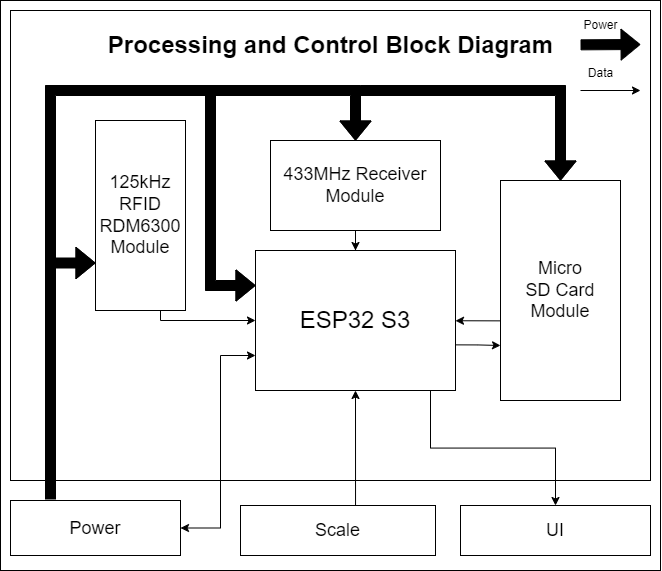
\includegraphics[width=0.5\textwidth]{../Figures/BD.png}
    \caption{Block Diagram}
    \label{fig:BD}
\end{figure}

\begin{figure}[htbp]
    \centering
    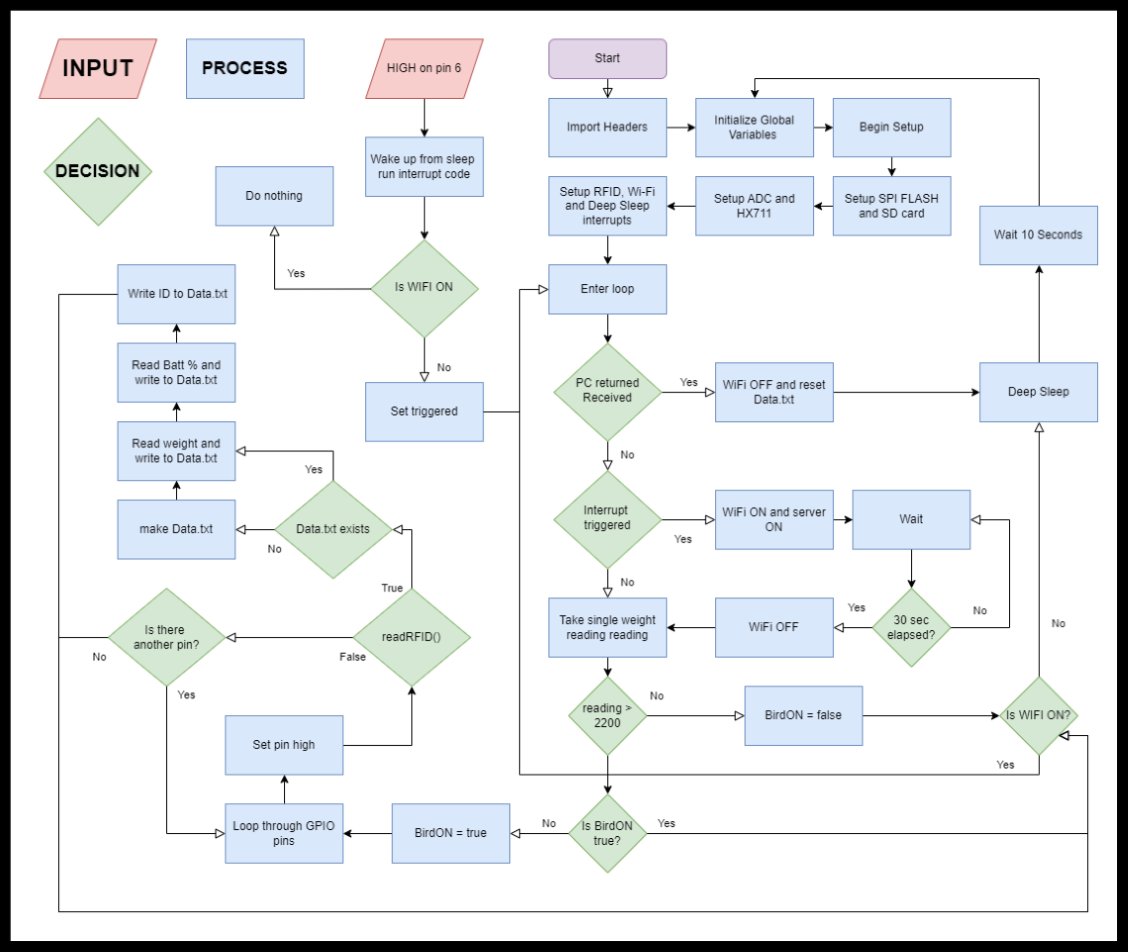
\includegraphics[width=1\textwidth]{../Figures/FC.png}
    \caption{System Control Flowchart}
    \label{fig:FC}
\end{figure}

\subsection*{Circuit Diagram}

\begin{figure}[htbp]
    \centering
    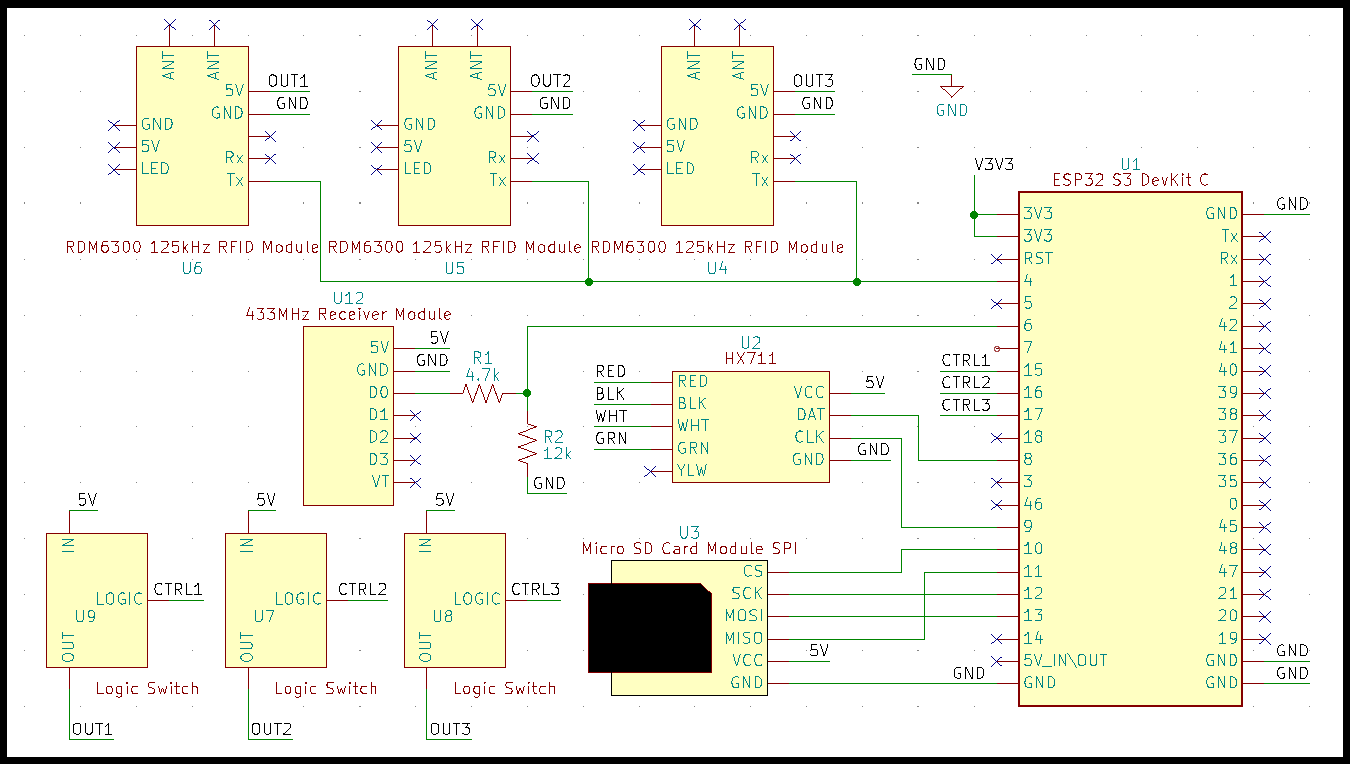
\includegraphics[width=1\textwidth]{../Figures/Circuit.png}
    \caption{Circuit Diagram}
    \label{fig:CD}
\end{figure}

\subsection*{Used Libraries}
The following libraries are not part of the stand C libraries or standard Arduino libraries, but were used in the final code. Table \ref{tab}

\begin{table}[htbp]
    \centering
    \adjustbox{width=\textwidth}
    {\begin{tabular}{|l|p{0.6\linewidth}|l|}
        \hline
        \textbf{Header File} & \textbf{Description} & \textbf{Author} \\
        \hline
        HX711.h & Description of HX711.h & Author A \\
        AsyncTCP.h & Description of AsyncTCP.h & Author B \\
        ESPAsyncWebServer.h & Description of ESPAsyncWebServer.h & Author C \\
        \hline
    \end{tabular}}
    \caption{External Libraries}
    \label{tab:extL}
\end{table}

\subsection*{Custom RFID Reading}
\subsection*{Weight Processing Results}

\section{ATP Results}

\section{Conclusions and Recommendations}

The Processing and Control subsystem contains the central processing unit of the entire system and acts as a cnetral hub for data while in the field. In this iteration, weight data and RFID data was succesfully collected, stored in a micro SD card and upon an external remote button press, transmitted to the user device via WiFi. Weight processing techniques were investigated and it was found that the median filter performs best. 
% ----------------------------------------------------
\ifstandalone
    \bibliography{../Bibliography/References.bib}
    % \printnoidxglossary[type=\acronymtype,nonumberlist]
\fi
\end{document}
% ----------------------------------------------------